\documentclass[journal]{IEEEtran}
\usepackage[T1]{fontenc}
\usepackage[utf8]{inputenc}
\usepackage{cite}
\usepackage{amsmath,amssymb}
\usepackage{graphicx}
\usepackage{booktabs}
\usepackage{multirow}
\usepackage{array}
\usepackage{tabularx}
\usepackage{algorithm}
\usepackage{algpseudocode}
\usepackage{url}
\usepackage{xcolor}

\setlength{\textfloatsep}{7pt plus 1pt minus 2pt}
\setlength{\floatsep}{7pt plus 1pt minus 2pt}
\setlength{\intextsep}{7pt plus 1pt minus 2pt}
\setlength{\abovecaptionskip}{3pt}
\setlength{\belowcaptionskip}{0pt}
\setlength{\abovedisplayskip}{5pt plus 1pt minus 2pt}
\setlength{\belowdisplayskip}{5pt plus 1pt minus 2pt}
\renewcommand{\textfraction}{0.08}
\renewcommand{\topfraction}{0.92}
\renewcommand{\dbltopfraction}{0.92}
\renewcommand{\floatpagefraction}{0.8}
\renewcommand{\dblfloatpagefraction}{0.8}
\newcolumntype{Y}{>{\raggedright\arraybackslash}X}
\newcolumntype{L}[1]{>{\raggedright\arraybackslash}p{#1}}
\raggedbottom

\title{Does Route Choice Matter in Ride-Pooling Dispatch?\\Spatiotemporal Corridor Matching on Public Taxi Data}
\author{Anonymous Authors}

\begin{document}
\maketitle
\vspace{-1.0em}

\begin{abstract}
Route choice in ride-pooling is usually treated as a routing detail or absorbed into a larger dispatch optimizer, even though different feasible paths expose the platform to different rider pools and therefore different matching outcomes. This paper studies route-aware dispatch through a matching-ball pipeline that combines H3 corridor construction, exact post-retrieval request-time filtering, feasibility screening, route scoring, and rolling-horizon evaluation. For each driver origin--destination pair, the system requests three genuine OSRM alternatives, builds route-specific H3 corridors, retrieves candidate riders through coarse spatiotemporal indexing, and then enforces exact time compatibility and route feasibility before policy scoring.

The empirical study uses public NYC Yellow and Green Taxi data, with long trips as proxy drivers and shorter trips as proxy rider requests. Riders are pre-sampled to 25\% for tractable offline simulation, indexed with 15-minute H3 bins for retrieval speed, and filtered afterward by an exact request window. The main dispatch experiment embeds route selection inside a 60-second rolling-horizon simulator with rider exclusivity and one-step conflict recomputation. In the Yellow 10\% retained-sample sparse regime, cold-start incurs \(\$8.08\) loss per launched driver, the strongest non-ML heuristic reduces that loss to \(\$7.30\), ML warm-up reduces it to \(\$7.15\), and the oracle within the route set reaches \(\$7.02\). Thus the route-aware layer reduces operating loss by \(\$0.93\) relative to cold-start, while ML retains a smaller \(\$0.15\) edge over the strongest heuristic. The same qualitative ordering is preserved in the Green public-domain robustness run.

We complement the system-level dispatch results with a larger controlled single-driver study as \emph{secondary evidence} that isolates route-ranking effects. Across both evaluation layers, most of the route-aware gain is already recovered by strong heuristics, while the learned scorer adds a smaller residual improvement. On temporal holdout, the tuned Yellow LightGBM model reaches \(R^2=0.801\) and RMSE \(=\$5.85\); the Green counterpart reaches \(R^2=0.738\) and RMSE \(=\$2.73\). The paper's central conclusion is therefore not that ML dominates dispatch, but that route-aware candidate construction and realism-first timing materially alter dispatch conclusions, while learned ranking provides a smaller but consistent gain over strong rule-based policies.
\end{abstract}

\begin{IEEEkeywords}
ride-pooling, dispatch, route selection, spatiotemporal matching, H3, OSRM, profit prediction, intelligent transportation systems
\end{IEEEkeywords}

\section{Introduction}
\IEEEPARstart{R}{ide}-pooling systems make route and dispatch decisions under tight latency constraints. In most production-style workflows, a driver is committed to the default route returned by a routing engine, usually the fastest or lowest-cost path. That cold-start policy ignores an operational fact: alternative routes expose the platform to different rider neighborhoods, different time-compatible requests, and different post-matching economics. If the platform can score a small set of genuine road-network alternatives before commitment, route choice becomes a dispatch lever rather than a passive routing detail.

This paper studies that lever through \emph{matching-ball dispatch}. For each driver trip, the platform requests three genuine OSRM alternatives, builds an H3 corridor around each route, retrieves riders whose pickup and drop-off remain compatible with that corridor, and ranks the routes with either rule-based heuristics or a learned route-value model. Unlike earlier implementations that effectively treat coarse lookup bins as the matching rule, the present study separates retrieval speed from eligibility. Fifteen-minute H3/time bins are used only to narrow the search; riders remain in the candidate set only if their true pickup timestamps satisfy an exact request-offset rule.

The paper also moves beyond isolated route scoring. The main experiment is a 60-second rolling-horizon dispatch simulator in which active drivers compete for a shared pool of open requests, rider exclusivity is enforced greedily inside each batch, and later drivers are recomputed once against the reduced pool before launch. That system-level evidence is paired with a larger controlled single-driver study that isolates route-choice effects without dispatch conflict. Together, these two views answer complementary questions: does route-aware warm-up help in a shared dispatch environment, and how much of the remaining headroom comes from route ranking itself rather than competition for overlapping riders?

The main contributions are:
\begin{enumerate}
    \item A realism-first route-evaluation pipeline that separates coarse H3/time retrieval from exact request-time eligibility.
    \item A route-aware matching-ball method that combines H3 corridor construction, one-ring expansion, exact request filtering, directionality, detour control, and greedy seat assignment into one reproducible retrieval-and-scoring layer.
    \item A dispatch-first evaluation in which route warm-up is embedded inside a 60-second rolling-horizon multi-driver simulator, with public cross-domain robustness on NYC Yellow and NYC Green Taxi data.
    \item A stronger baseline study showing that most of the system-level gain comes from route-aware retrieval versus cold-start, while the learned route ranker provides only a modest edge over the strongest non-ML heuristic and a simple path-buffer comparator.
\end{enumerate}

Section II reviews related work. Section III describes the data and proxy construction. Section IV introduces the matching-ball retrieval and route-ranking layer. Section V describes the rolling dispatch simulator. Section VI details the experimental design. Section VII presents system-level and controlled results. Section VIII discusses limitations and publication-facing positioning. Section IX concludes.

\section{Related Work}
Dynamic ride-sharing and ride-pooling have been studied from the perspectives of assignment, optimization, and feasibility. Alonso-Mora \emph{et al.} cast high-capacity ride-sharing as dynamic trip--vehicle assignment and showed the value of optimization at scale \cite{alonso2017}. Agatz \emph{et al.} surveyed dynamic ride-sharing formulations and emphasized the interaction between temporal constraints and operational trade-offs \cite{agatz2012}; their earlier Atlanta study also showed that better decision rules can materially outperform naive greedy baselines \cite{agatz2011}. Stiglic \emph{et al.} quantified the role of driver and rider flexibility in dynamic ride-sharing feasibility \cite{stiglic2016}.

Timing assumptions are especially important in pooling studies. Santi \emph{et al.} quantified shareability under short temporal windows and showed that compatibility assumptions materially affect estimated pooling opportunity \cite{santi2014}. Tachet \emph{et al.} further showed that ride-sharing feasibility scales rapidly with density when the delay window remains small \cite{tachet2017}. Those results motivate our explicit distinction between coarse retrieval bins and exact request-time eligibility.

Ride-hailing dispatch has since grown into a large literature spanning order assignment, multi-driver coordination, repositioning, and reinforcement learning. Learning-and-planning dispatch policies have been studied for large ride-hailing platforms \cite{xu2018dispatch}, including deep value-network dispatch \cite{tang2019deepvalue}, multi-agent fleet management \cite{lin2018fleet}, mean-field ridesharing dispatch \cite{li2019meanfield}, multi-agent order--vehicle distribution matching \cite{zhou2019ovdm}, and joint order-dispatching / fleet-management formulations \cite{jin2019coride}, and unified value-function frameworks \cite{tang2021value}. Queueing-theoretic dispatch models \cite{cheng2019queueing} and practical online driver repositioning systems \cite{xu2020reposition} further show that system-level outcomes depend strongly on how matching and geographic exposure are coupled over time. Pickup-and-delivery and vehicle-routing perspectives \cite{berbeglia2010dynamic,pillac2013dynamic,psaraftis1995dynamic,solomon1987vrptw,laporte2009fifty,toth2002vrp,savelsbergh1995general,cordeau2007dialaride} formalize temporal feasibility and path structure in ways that motivate separating fast retrieval from exact screening. Fleet-scale analyses \cite{vazifeh2018fleet,braverman2019empty} and stochastic matching formulations \cite{bertsimas2019online,ozkan2020dynamic} likewise emphasize idle routing and supply--demand imbalance as first-class controls. Learning-based dispatch, repositioning, and rebalancing \cite{wang2020knowledge,ding2020rebalancing,wei2024repositioning,mao2020avdispatch,wallar2019routing,lei2023rlpricing,liu2022personalizedroute} parallel platform practice \cite{xu2020reposition}, while recent ride-pooling traffic and pricing studies \cite{ke2020ridepooling,karaenke2023expool} connect operational rules to congestion and revenue management. Our paper does not attempt to replace that broader fleet-optimization literature. It focuses on a narrower question that those studies usually absorb into a larger optimizer: whether route choice itself changes the candidate pool enough to matter operationally.

Route recommendation has also been studied as a matching-quality lever rather than only a routing problem. Ma \emph{et al.} developed T-Share, a large-scale dynamic taxi ridesharing service with spatiotemporal indexing \cite{ma2013tshare}. Bassem \emph{et al.} explored route recommendation for carpool facilitation \cite{bassem2022}, while Xia \emph{et al.} showed that route structure itself affects matching outcomes in joint social and route networks \cite{xia2019}. In ride-service operations, systematic search and tree-based optimization have been used to improve online decisions \cite{chen2021}. More recent work has pushed toward jointly optimizing matching, routing, and pickup/drop-off design in rolling-horizon settings \cite{stumpe2024,zhou2026}. Those studies motivate our route-aware formulation, but our methodological emphasis is different: we separate route-aware candidate construction from exact-time eligibility and ask how much of the resulting lift survives inside a lightweight dispatch layer.

Recent ride-hailing work has also highlighted fairness and system design concerns beyond pure efficiency \cite{suhr2019fair,shi2021fair,raman2021fair}. We do not model fairness or repositioning explicitly here, and we therefore avoid claiming a full fleet-management solution. Instead, the paper contributes a reproducible public-data benchmark for route-aware candidate construction under realistic timing assumptions.

Methodologically, the implementation uses H3 spatial indexing \cite{h3docs}, OSRM route alternatives \cite{osrmapi}, and gradient-boosted trees via LightGBM \cite{ke2017} and XGBoost \cite{chen2016xgboost}, with comparison baselines that include a linear regressor, LambdaRank, and a neural network. The novelty is therefore not ``use ML on taxi data,'' but to combine route-aware retrieval, realism-first timing, and system-level dispatch evaluation in one reproducible package.

\section{Data and Proxy Construction}
\subsection{Public Domains}
We use the NYC Yellow Taxi and NYC Green Taxi public datasets from Azure Open Datasets \cite{azureyellow,azuregreen,azuredocs}. The retained columns include trip timestamps, pickup and drop-off coordinates, trip distance, fare amount, total amount, tips, and passenger count. Table~\ref{tab:data_split} summarizes the temporal split: January--February 2015 are used for training, March 2015 for temporal validation and model selection, and April 2015 for policy evaluation. Green data are used as a public second domain rather than a second city; the goal is cross-domain robustness under similar exact-point telemetry, not a forced intercity comparison with degraded coordinates.

\begin{table}[!t]
\caption{Temporal split used in both public domains.}
\label{tab:data_split}
\centering
\footnotesize
\begin{tabularx}{\columnwidth}{L{0.18\columnwidth}L{0.28\columnwidth}Y}
\toprule
Role & Months & Purpose \\
\midrule
Training & January--February 2015 & Model fitting and historical summaries \\
Validation & March 2015 & Temporal holdout selection and calibration \\
Evaluation & April 2015 & Dispatch and paired-policy experiments \\
\bottomrule
\end{tabularx}
\end{table}

\subsection{Proxy Roles and Retained-Sample Semantics}
Trips are partitioned into:
\begin{itemize}
    \item \textbf{Drivers:} trips longer than 10 miles.
    \item \textbf{Riders:} trips from 0.5 to 10 miles.
\end{itemize}

Riders are pre-sampled to 25\% before any density sweep. This is a tractability choice for the public benchmark, not a claim about full market share. Throughout the paper, \emph{100\% density} therefore means the full retained 25\% rider sample, not full city demand.

\subsection{Proxy Validity and Scope}
The proxy construction deserves explicit scope calibration. The retained taxi trips are not native pooled requests, and the platform-side economics do not encode rider acceptance, cancellation, or driver repositioning behavior. The proxy is nonetheless useful for the narrower question studied here because it preserves exact pickup/drop-off coordinates, timestamps, trip distances, and fare magnitudes at city scale under a fully public benchmark. In other words, the proxy is appropriate for relative comparison of route-aware candidate construction, exact-time eligibility, and route-ranking policies under controlled assumptions. It is not appropriate for claiming true market adoption rates, platform-wide profitability, or behavioral response to pooling incentives.

\subsection{Scenario Assumptions}
Reported values are \emph{scenario profit} outputs under fixed assumptions. Table~\ref{tab:scenario_assumptions} summarizes the primary configuration and the sensitivity ranges used later in the paper. These settings support controlled comparison; they are not calibrated platform margins.

\begin{table}[!t]
\caption{Scenario assumptions and operating regimes used throughout the paper.}
\label{tab:scenario_assumptions}
\centering
\footnotesize
\begin{tabularx}{\columnwidth}{L{0.26\columnwidth}L{0.22\columnwidth}Y}
\toprule
Component & Primary value & Notes / sweep \\
\midrule
Indexing cadence & 15-minute bins, \(\pm1\) adjacent bins & Retrieval only; not the final eligibility rule \\
Exact request window & 5 minutes & Sensitivity: \(\{2,5,10\}\) minutes \\
Maximum detour & 4 minutes & Sensitivity: \(\{2,4,6\}\) minutes \\
Retained-sample density & 10\% headline sparse regime & Density sweep: \(\{100,25,10\}\)\% of the pre-sampled rider pool \\
Seat capacity & 3 seats per driver & Fixed across all experiments \\
Platform share & \(\alpha=0.50\) & Scenario-profit assumption \\
Driving cost & \(c=\$0.67\) per mile & Scenario-profit assumption \\
Urban speed proxy & 40 km/h & Converts geometric detour into minutes \\
\bottomrule
\end{tabularx}
\end{table}

\begin{figure*}[!t]
\centering
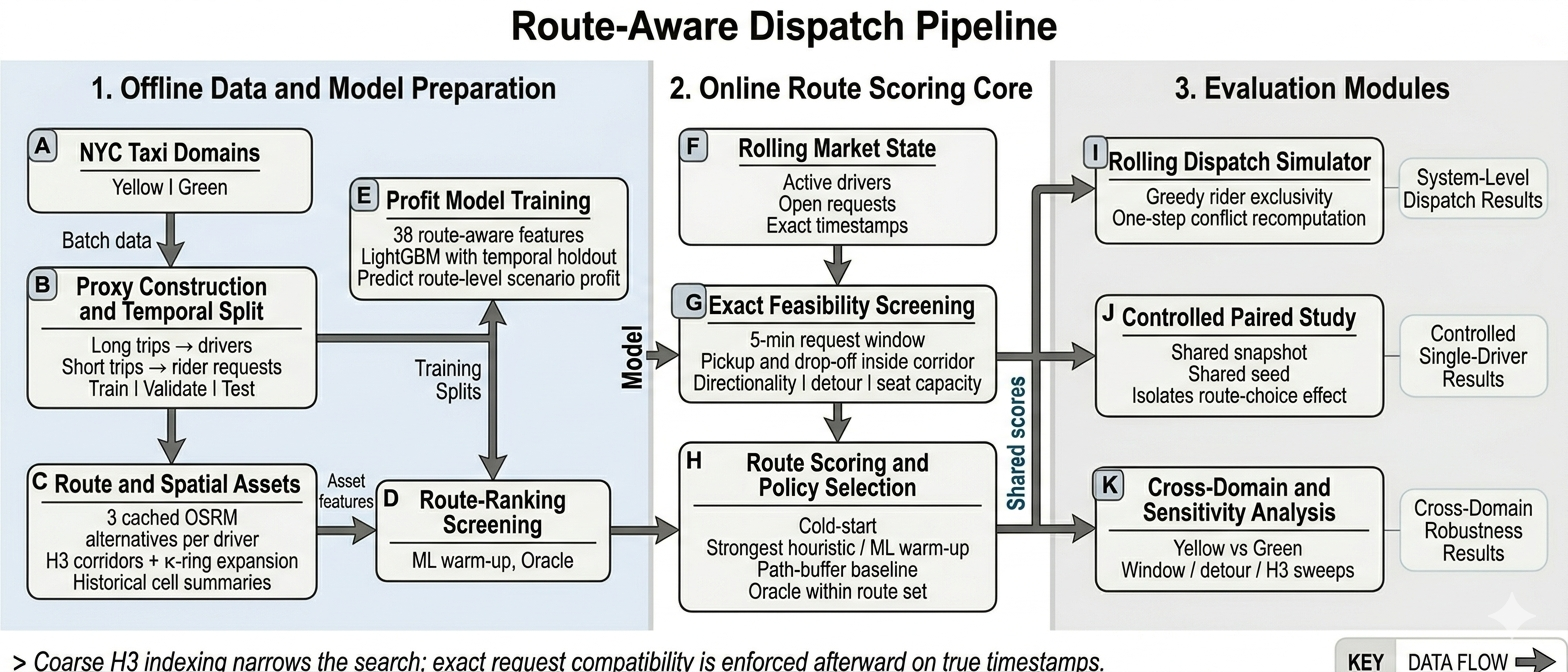
\includegraphics[width=\textwidth]{figures/paper_fig1_dispatch_architecture_v2.png}
\caption{Dispatch-first system architecture. The figure separates offline asset construction from online route scoring and from the two evaluation branches used in the paper. The key methodological distinction is that H3 corridors and 15-minute bins are used only to narrow the search, whereas exact request compatibility and route feasibility are enforced afterward before policy scoring.}
\label{fig:dispatch_architecture}
\end{figure*}

\section{Matching-Ball Retrieval and Route Ranking}
Figure~\ref{fig:dispatch_architecture} summarizes the paper's end-to-end pipeline, and Table~\ref{tab:notation} collects the notation used throughout this section. Public taxi trips are converted into proxy drivers and riders, each driver receives three genuine route alternatives, matching-ball retrieval narrows the candidate pool through H3 corridors and coarse time bins, and exact request compatibility is enforced only after retrieval. The resulting route scores then feed both the rolling dispatch simulator and the larger single-driver paired study.

\begin{table}[!t]
\caption{Notation used in the matching-ball and dispatch formulation.}
\label{tab:notation}
\centering
\footnotesize
\begin{tabularx}{\columnwidth}{L{0.30\columnwidth}Y}
\toprule
Symbol & Meaning \\
\midrule
\(d \in \mathcal{D}\) & Driver trip in the evaluation set \\
\(u \in \mathcal{U}\) & Rider request \\
\(\mathcal{R}_d=\{r_{d1},\dots,r_{dK}\}\) & Candidate route set for driver \(d\), with \(K=3\) in the paper \\
\(\pi_r\) & Polyline of route \(r\) returned by OSRM \\
\(R_r\) & Ordered H3 spine obtained by densifying \(\pi_r\) and mapping it to H3 cells \\
\(C_r\) & Matchable H3 corridor derived from \(R_r\) \\
\(h_u^{p}, h_u^{q}\) & Pickup and drop-off H3 cells of rider \(u\) \\
\(t_d, t_u\) & Driver departure timestamp and rider pickup timestamp \\
\(\tau_{\mathrm{req}}, \tau_{\mathrm{det}}\) & Exact request-time and detour thresholds \\
\(\mathcal{U}_r^{\mathrm{cand}}, \mathcal{U}_r^{\mathrm{feas}}\) & Retrieved candidate set and exact-feasible rider set for route \(r\) \\
\(M_r\) & Matched rider set produced for route \(r\) after greedy seat assignment \\
\(s_\phi(d,r)\) & Route score under policy \(\phi\) \\
\(g(d,r)\) & Realized scenario profit for assigning driver \(d\) to route \(r\) \\
\(\mathcal{U}_b\) & Open request pool at dispatch batch \(b\) \\
\bottomrule
\end{tabularx}
\end{table}

\subsection{H3 Corridor Construction}
Each driver origin--destination pair is routed through OSRM \cite{osrmapi}. The implementation stores a persistent route cache so that evaluation does not depend on live API latency once the cache is populated. For each driver \(d\), three genuine road-network alternatives are requested. Every route polyline \(\pi_r\) is densified at 80 m spacing and mapped to ordered H3 resolution-9 cells \cite{h3docs}. Let \(R_r=(h_1,\dots,h_m)\) denote the ordered H3 cells traversed by route \(r\). The matchable corridor is
\[
C_r=\bigcup_{h\in R_r}\mathrm{Disk}_{\kappa}(h),
\]
where \(\mathrm{Disk}_{\kappa}(h)\) is the H3 \(\kappa\)-ring neighborhood around cell \(h\). The primary configuration uses \(\kappa=1\), i.e., \(\mathrm{Disk}_1(h)\); later sensitivity analysis varies corridor width to show how retrieval geometry changes both the candidate pool and the ranking difficulty.

\subsection{Exact-Time Matching-Ball Retrieval}
Retrieval is intentionally two-stage. Each rider is indexed by pickup cell, drop-off cell, service date, and 15-minute pickup bin. At query time, the route contributes its corridor cells \(C_r\), and the retrieval step searches the driver's departure bin plus adjacent bins on the same service date only as a coarse speed device. The coarse candidate set for route \(r\) is
\begin{equation}
\small
\mathcal{U}_r^{\mathrm{cand}}=
\left\{
u\in\mathcal{U}\ \middle|\
\begin{aligned}
&h_u^{p}\in C_r,\ h_u^{q}\in C_r,\\
&\beta(t_u)\in\{\beta(t_d)-1,\beta(t_d),\beta(t_d)+1\},\\
&\delta_u=\delta_d
\end{aligned}
\right\}.
\normalsize
\end{equation}
Here \(\beta(\cdot)\) maps a timestamp to its 15-minute bin and \(\delta_u\) is the service date. Exact eligibility is then enforced on the true pickup timestamp:
\[
|t_u - t_d| \le \tau_{\mathrm{req}},
\]
with \(\tau_{\mathrm{req}}=5\) minutes in the primary scenario.

The exact-feasible set is therefore
\begin{equation}
\small
\mathcal{U}_r^{\mathrm{feas}}=
\left\{
u\in\mathcal{U}_r^{\mathrm{cand}}\ \middle|\
\begin{aligned}
&|t_u-t_d|\le\tau_{\mathrm{req}},\\
&\psi_r(u)=1,\ \Delta_r(u)\le\tau_{\mathrm{det}},\\
&p_u\le s_d
\end{aligned}
\right\}.
\normalsize
\end{equation}
Here \(\psi_r(u)\) is a directionality-validity indicator, \(\Delta_r(u)\) is detour in minutes, \(p_u\) is rider party size, and \(s_d\) is remaining seat capacity. Matching-ball retrieval is therefore route-aware, date-aware, and exact-time eligible even though coarse bins are used for indexing speed.

\begin{figure*}[!t]
\centering
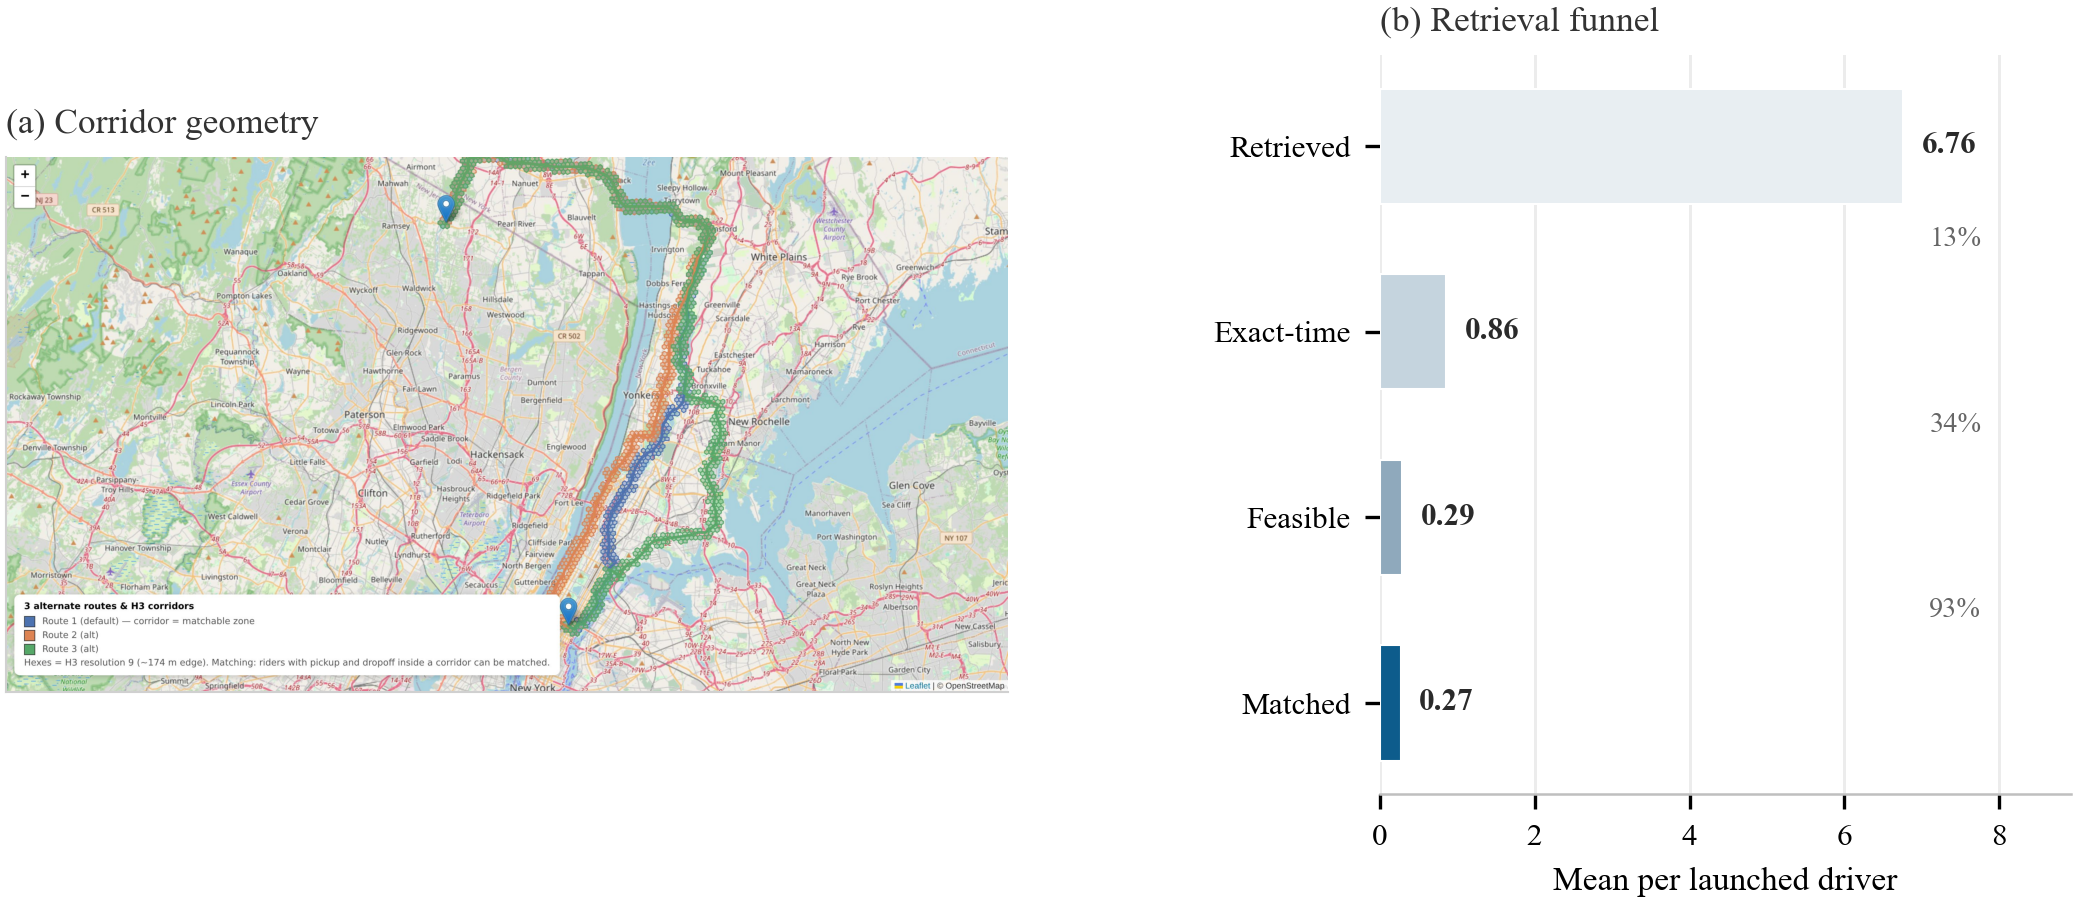
\includegraphics[width=\textwidth]{figures/paper_fig2_matching_ball_mechanism.png}
\caption{Matching-ball mechanism. Panel (a) depicts the \emph{spatial} layer of matching-ball retrieval: densified OSRM alternatives are converted into route-specific H3 corridors whose one-ring expansion creates buffered candidate space rather than a generic hotspot lookup. The map alone does not encode the time window or feasibility rules; those are applied afterward. Panel (b) shows the Yellow 10\% stress-test dispatch funnel for the warm-up policy: retrieved corridor candidates average 6.76 per launched driver, 0.86 remain dispatch-available after exact-time filtering, 0.29 survive detour/seat feasibility, and 0.27 are finally matched riders.}
\label{fig:matching_ball}
\end{figure*}

Figure~\ref{fig:matching_ball} makes the realism contribution concrete. The retrieved corridor candidates are numerous enough to justify route-aware retrieval, but only a small subset remain simultaneously open in the request pool and exact-window compatible at the driver's actual departure time. In the Yellow 10\% stress-test scenario, only about 13\% of retrieved corridor candidates survive that dispatch-availability filter, and only a smaller subset of those survive detour and seat checks. Matching-ball retrieval is therefore both route-aware and realism-first.

\subsection{Route-Ranking Policies}
Among feasible riders, seat assignment is greedy by fare with seed-controlled tie-breaking. Let \(\Gamma(\mathcal{U}_r^{\mathrm{feas}},s_d)\) denote that greedy seat-assignment operator, so that \(M_r=\Gamma(\mathcal{U}_r^{\mathrm{feas}},s_d)\). For route \(r\), realized scenario profit is
\[
g(d,r)= \alpha \sum_{u\in M_r}f_u - c\cdot \ell_r,
\]
where \(f_u\) is rider fare, \(\alpha\) is platform share, \(c\) is cost per mile, and \(\ell_r\) is route distance in miles. Policies differ only in the route score \(s_\phi(d,r)\) used to select
\[
r_d^\phi=\arg\max_{r\in\mathcal{R}_d}s_\phi(d,r).
\]

\begin{table}[!t]
\caption{Route-selection policies and score definitions.}
\label{tab:policy_definitions}
\centering
\footnotesize
\begin{tabularx}{\columnwidth}{L{0.24\columnwidth}Y L{0.18\columnwidth}}
\toprule
Policy & Score definition \(s_\phi(d,r)\) & Deployable online? \\
\midrule
Cold-start & Indicator for the first OSRM route & Yes \\
Random & Uniform draw over \(\mathcal{R}_d\) & Yes \\
Heuristic count & \(|\mathcal{U}_r^{\mathrm{cand}}|\) & Yes \\
Heuristic fare density & Corridor fare density summary & Yes \\
Heuristic feasible count & \(|\mathcal{U}_r^{\mathrm{feas}}|\) & Yes \\
Heuristic profit proxy & Hand-built non-ML value proxy & Yes \\
ML warm-up & Predicted scenario profit \(\hat g(d,r)\) & Yes \\
Oracle (route set) & Realized scenario profit \(g(d,r)\) & No \\
\bottomrule
\end{tabularx}
\end{table}

Table~\ref{tab:policy_definitions} lists all route-selection policies. The strongest non-ML heuristic is selected from the four rule-based policies within each reported scenario. In the primary dispatch scenario, the selected heuristic is feasible-rider count.

\section{Rolling-Horizon Dispatch Design}
The main paper contribution is not only route ranking in isolation, but route ranking embedded inside a shared rider pool. We therefore add a rolling-horizon dispatch simulator with 60-second batching. Let \(\mathcal{U}_b\) denote the open request pool at batch \(b\). Drivers are scored route-by-route against \(\mathcal{U}_b\), and each policy produces a provisional score
\[
\omega_d^\phi=s_\phi\!\left(d,r_d^\phi\right),
\]
where \(r_d^\phi\) is the provisional best route for driver \(d\) under policy \(\phi\). Active drivers in the batch are processed in descending \(\omega_d^\phi\), with deterministic fallback to departure time.

When a driver is finalized, the corresponding matched riders are removed from the pool:
\[
\mathcal{U}_b^{(j+1)}=\mathcal{U}_b^{(j)}\setminus M_{r_{d_j}^{\phi}},
\]
where \(d_j\) is the \(j\)-th driver in batch order. The next driver is then re-evaluated once against \(\mathcal{U}_b^{(j+1)}\). This one-step conflict recomputation is sufficient to enforce rider exclusivity while keeping the simulation low latency. Algorithm~\ref{alg:dispatch} formalizes the full batch loop.

\begin{algorithm}[!t]
\caption{Route-aware retrieval and scoring for one driver}
\label{alg:route_scoring}
\footnotesize
\begin{algorithmic}[1]
\Require Driver \(d\), route set \(\mathcal{R}_d\), policy \(\phi\)
\Statex \hspace{\algorithmicindent} Open request pool \(\mathcal{U}_b\)
\ForAll{\(r \in \mathcal{R}_d\)}
    \State Build corridor \(C_r\) from the densified route spine
    \State Retrieve \(\mathcal{U}_r^{\mathrm{cand}}\) from the H3/time index
    \State Filter to \(\mathcal{U}_r^{\mathrm{feas}}\) using
    \Statex \hspace{\algorithmicindent} exact time, directionality, detour, and seats
    \State Compute \(M_r=\Gamma(\mathcal{U}_r^{\mathrm{feas}},s_d)\) by greedy seat assignment
    \State Compute realized route value \(g(d,r)\) and policy score \(s_\phi(d,r)\)
\EndFor
\State \Return \(r_d^\phi=\arg\max_{r \in \mathcal{R}_d}s_\phi(d,r)\)
\end{algorithmic}
\end{algorithm}

\begin{algorithm}[!t]
\caption{Rolling-horizon dispatch with one-step conflict recomputation}
\label{alg:dispatch}
\footnotesize
\begin{algorithmic}[1]
\Require Batched driver stream, batched rider stream
\Statex \hspace{\algorithmicindent} Policy \(\phi\)
\State Initialize open request pool \(\mathcal{U}_b \gets \emptyset\)
\For{each dispatch batch \(b\)}
    \State Add newly observed riders to \(\mathcal{U}_b\)
    \State Remove riders whose exact request window has elapsed
    \State Activate drivers whose departure times fall inside batch \(b\)
    \ForAll{active drivers \(d\)}
        \State Compute provisional route \(r_d^\phi\) using Algorithm~\ref{alg:route_scoring}
        \State Set ordering score \(\omega_d^\phi=s_\phi(d,r_d^\phi)\)
    \EndFor
    \State Sort active drivers by descending \(\omega_d^\phi\), breaking ties by departure time
    \ForAll{sorted drivers \(d_j\)}
        \State Recompute route scores once against the current pool \(\mathcal{U}_b^{(j)}\)
        \State Finalize \(r_{d_j}^{\phi}\) and matched set \(M_{r_{d_j}^{\phi}}\)
        \State Update \(\mathcal{U}_b^{(j+1)} \gets \mathcal{U}_b^{(j)} \setminus M_{r_{d_j}^{\phi}}\)
        \State Remove launched driver \(d_j\) from the active set
    \EndFor
\EndFor
\end{algorithmic}
\end{algorithm}

This is still a dispatch approximation. It does not reposition vehicles, optimize global assignment over long horizons, or keep launched drivers active after commitment. Once a driver launches on a route, that driver exits the batch system. The simulator should therefore be read as a low-latency route-choice layer embedded in a rolling shared-request environment, not as a full production dispatch platform.

\section{Experimental Design}
\subsection{System-Level Dispatch}
The dispatch experiments use 1000 April 2015 Yellow test drivers and five seeds. Repeat-run summaries are aggregated at the seed level before reporting intervals across retained-sample seeds, although many of those intervals collapse visually because the simulator is nearly deterministic once the retained rider sample is fixed. These intervals should therefore be read as repeat-run dispersion under the retained-sample protocol rather than as broad inferential uncertainty. The headline dispatch assumptions are:
\begin{itemize}
    \item domain = Yellow,
    \item batch cadence = 60 seconds,
    \item retained-sample density = 10\%,
    \item exact request window = 5 minutes,
    \item max detour = 4 minutes.
\end{itemize}

Additional dispatch sweeps vary density \(\{100,25,10\}\), request window \(\{2,5,10\}\) minutes, and detour \(\{2,4,6\}\) minutes. The public second-domain experiment repeats the 10\% stress-test dispatch scenario and density sweep on Green using the same January--February 2015 train, March 2015 validation, April 2015 test structure.

\subsection{Controlled Single-Driver Analysis}
The isolated-driver paired analysis uses 5{,}000 April Yellow test drivers and five seeds. Each strategy sees the same driver, rider snapshot, route set, and random seed; only the route-selection rule changes. This larger controlled study is retained because it isolates route-ranking effects without driver competition.

\subsection{Model Development and Metrics}
Yellow model development uses January--February 2015 for training and March 2015 for validation and selection; the final deployed Yellow model is retrained on January--March before April evaluation. The same temporal pattern is used for Green. The tuned model uses 38 features that exclude realized matching outputs, spanning geometry, temporal context, spatial demand, and landmark/cell context.

For a policy \(\phi\), the main reported system metrics are
\begin{equation}
\begin{aligned}
\bar g_\phi &= \frac{1}{|\mathcal{D}_\phi^{\mathrm{launch}}|}
\sum_{d \in \mathcal{D}_\phi^{\mathrm{launch}}} g(d,r_d^\phi),\\
\bar m_\phi &= \frac{1}{|\mathcal{D}_\phi^{\mathrm{launch}}|}
\sum_{d \in \mathcal{D}_\phi^{\mathrm{launch}}} |M_{r_d^\phi}|,
\end{aligned}
\end{equation}
that is, scenario profit per launched driver and matched riders per launched driver. Because \(\bar g_\phi\) is negative in the sparse regimes, the main presentation in the Results section emphasizes \emph{operating loss} and \emph{loss reduction} relative to cold-start rather than absolute profit creation.

We report:
\begin{itemize}
    \item \textbf{System metrics:} scenario profit per launched driver, operating loss per launched driver, rider service rate, mean wait, matched riders per driver, seat occupancy, and dispatch runtime.
    \item \textbf{Model metrics:} \(R^2\), RMSE, MAE, and route rank-1 accuracy.
    \item \textbf{Paired gaps:} mean driver-level differences, bootstrap confidence intervals, and win/tie/loss rates in the isolated-driver study.
\end{itemize}

\section{Results}
\subsection{Primary Yellow Sparse Dispatch}
Tables~\ref{tab:dispatch_primary} and \ref{tab:dispatch_delta} are the paper's main system-level results. Under 60-second batching, a 5-minute exact request window, and 10\% retained-sample density, route-aware policies materially improve over cold-start even in a thin rider market. ML warm-up again yields the best realizable policy, although the margin over the strongest heuristic remains modest and comes from better route-value tradeoffs rather than from serving strictly more riders.

\begin{table}[!t]
\caption{Primary Yellow sparse dispatch outcomes: 60-second batches, 5-minute exact request window, 10\% retained-sample density, 4-minute detour, 1000 drivers, five seeds.}
\label{tab:dispatch_primary}
\centering
\scriptsize
\setlength{\tabcolsep}{2.6pt}
\begin{tabular}{lrrrr}
\toprule
Policy & Loss/driver (\$) & Loss reduction & Matched/driver & Wait (min) \\
\midrule
Cold-start & 8.08 & --- & 0.16 & 2.51 \\
Best heuristic & 7.30 & 0.78 & 0.29 & 2.52 \\
ML warm-up & \textbf{7.15} & \textbf{0.93} & 0.27 & 2.56 \\
Oracle (route set) & 7.02 & 1.06 & 0.29 & 2.54 \\
\bottomrule
\end{tabular}
\end{table}

\begin{table}[!t]
\caption{Comparative interpretation of the primary Yellow sparse dispatch scenario.}
\label{tab:dispatch_delta}
\centering
\footnotesize
\begin{tabularx}{\columnwidth}{Yrr}
\toprule
Comparison & Delta (\$/driver) & Relative loss reduction \\
\midrule
Best heuristic vs.\ cold-start & +0.78 & 9.7\% \\
ML warm-up vs.\ cold-start & +0.93 & 11.5\% \\
Oracle vs.\ cold-start & +1.06 & 13.1\% \\
ML warm-up vs.\ best heuristic & +0.15 & 1.9\% \\
\bottomrule
\end{tabularx}
\end{table}

Two points matter. First, the route-aware layer clearly reduces operating loss relative to cold-start: \(\$0.93\) per launched driver, or about 11.5\% less loss in the sparse regime. Second, the learned ranker does \emph{not} dominate the strongest heuristic. Its edge is only \(\$0.15\) per driver, and the strongest heuristic actually matches slightly more riders. This is the right publication message: route-aware retrieval and ranking matter, while most of the system-level improvement is already captured by strong rule-based policies.

\subsection{Dispatch Density Response}
Figure~\ref{fig:dispatch_density} places the 10\% sparse headline result inside the full Yellow dispatch density sweep, plotting \emph{savings over cold-start} so the policy ordering is legible at every density level. At 10\% retained-sample density, the strongest heuristic saves \(\$0.78\) per launched driver relative to cold-start, ML warm-up saves \(\$0.93\), and the within-route-set oracle saves \(\$1.06\). At 25\%, the corresponding savings are \(\$1.24\), \(\$1.39\), and \(\$1.57\). At the full 100\% retained-sample benchmark, they are \(\$2.20\), \(\$2.31\), and \(\$2.75\). The route-aware layer consistently improves on cold-start at every density, and absolute savings grow as the rider pool densifies. The simulator is near-deterministic across seeds at fixed density; repeat-run variation is smaller than the marker size.

As a simple external-style sanity baseline, we also reran a 1 km path-buffer policy on a deterministic cached-route Yellow subset (250 drivers, five seeds) using the same exact-time and detour rules. That comparator improves upon cold-start but remains materially weaker than matching-ball retrieval. In dispatch at 10\%, the path-buffer policy reduces loss only from \(\$8.40\) to \(\$8.28\), whereas the paper's strongest matching-ball heuristic reaches \(\$7.30\). In the controlled single-driver study, the same path-buffer policy improves 25\% loss from \(\$5.59\) to \(\$4.40\), but still trails the paper-best matching-ball heuristic at \(\$3.53\). This sanity check does not replace a literature-grade external dispatch baseline, but it does show that the H3 corridor construction is not merely reproducing what a simple geometric buffer already captures.

\begin{figure*}[!t]
\centering
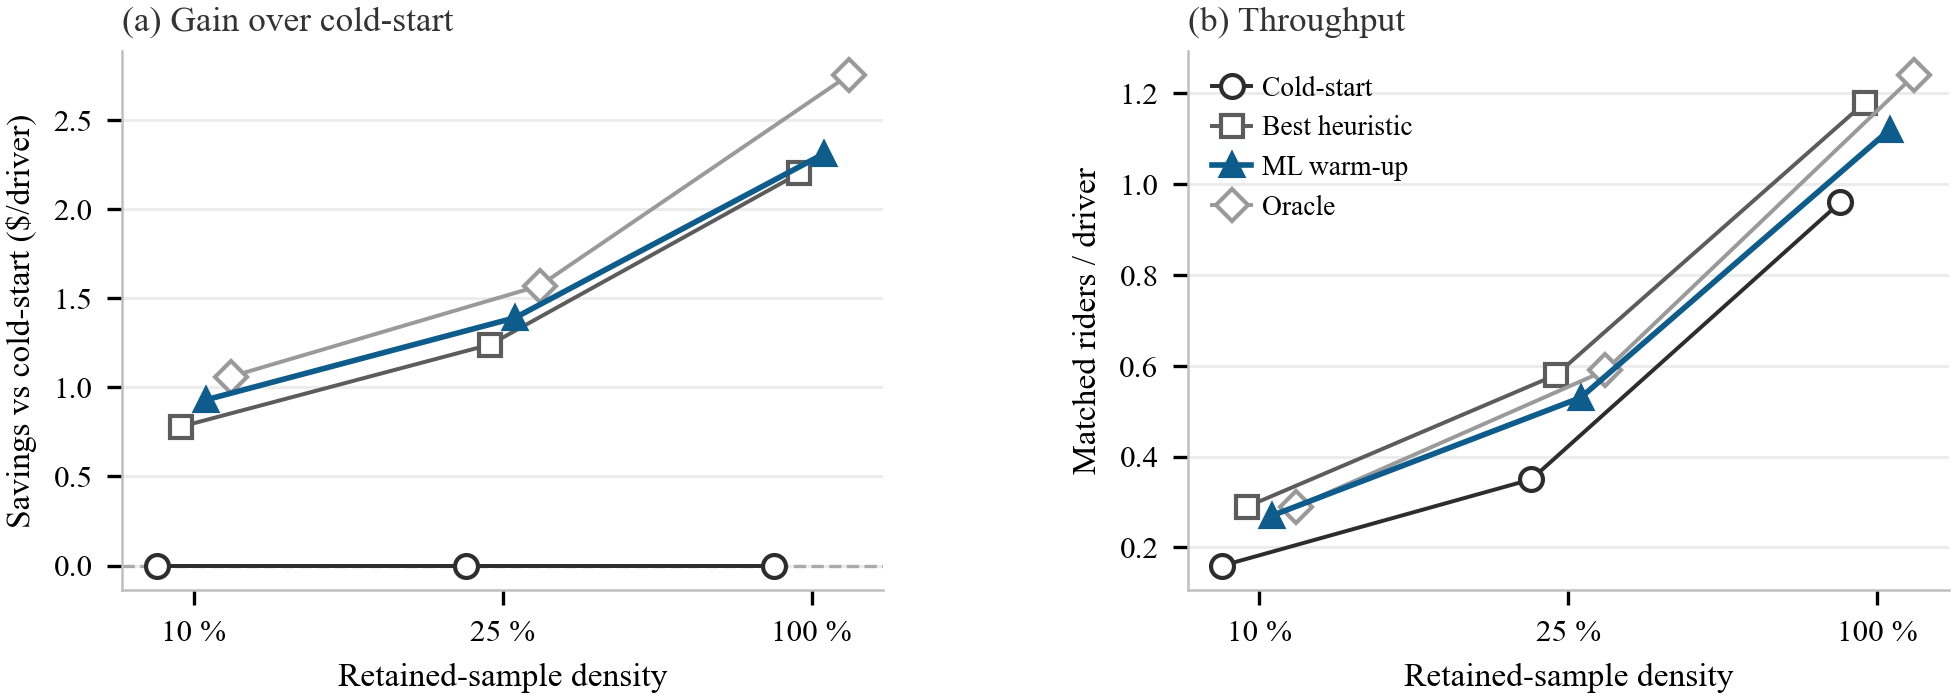
\includegraphics[width=\textwidth]{figures/paper_fig3_dispatch_density.png}
\caption{Dispatch density response under 60-second batches and a 5-minute exact request window. \emph{(a)} Savings over cold-start per launched driver (cold-start = \$0 reference line); plotting the \emph{gain} rather than the absolute loss spreads the policy lines and makes the ordering readable at every density. \emph{(b)} Matched riders per launched driver. The best heuristic leads ML warm-up in throughput at every density because it directly maximises compatible rider count (\texttt{heuristic\_feasible\_count}), whereas ML warm-up optimises route profit; the two objectives diverge slightly under sparse supply. The x-axis runs sparse (10\%) to dense (100\%), where 100\% refers to the full pre-sampled 25\% rider pool. The simulator is near-deterministic across seeds at fixed density; repeat-run variation is smaller than the marker size.}
\label{fig:dispatch_density}
\end{figure*}

\subsection{Cross-Domain Robustness}
Table~\ref{tab:domain_transfer} reports the public cross-domain comparison for the harsher 10\% stress-test regime. Green reproduces the same qualitative hierarchy as Yellow: cold-start is worst, warm-up is better, and the oracle within the route set remains the upper bound. The Green stress test is slightly less negative overall, and its wait times are lower.

\begin{table}[!t]
\caption{Stress-test dispatch scenario across public domains. Yellow and Green both use 60-second batching, a 5-minute exact request window, 10\% retained-sample density, 4-minute detour, 1000 drivers, and five seeds. Comparative deltas are interpreted relative to the domain-specific cold-start baseline.}
\label{tab:domain_transfer}
\centering
\scriptsize
\setlength{\tabcolsep}{2.4pt}
\begin{tabular}{lrrrr}
\toprule
Policy & Yellow loss & Green loss & Yellow wait & Green wait \\
\midrule
Cold-start & 8.08 & 7.66 & 2.51 & 1.87 \\
Best heuristic & 7.30 & 7.54 & 2.52 & 2.14 \\
ML warm-up & \textbf{7.15} & \textbf{7.27} & 2.56 & 2.07 \\
Oracle (route set) & 7.02 & 7.25 & 2.54 & 2.05 \\
\bottomrule
\end{tabular}
\end{table}

The warm-up edge over the strongest heuristic is \(\$0.15\) per launched driver in Yellow and \(\$0.27\) in Green. That is still a modest margin, but it survives the public-domain shift and therefore supports the paper's narrower, reviewer-safe claim: route-aware retrieval plus realistic timing help dispatch, and ML is a competitive route-ranker rather than a dramatic winner even under a harsher stress test.

\subsection{Controlled Single-Driver Mechanism}
The dispatch results answer the system question, but they do not isolate route-ranking effects. Figure~\ref{fig:single_driver_density} therefore compares the larger single-driver paired study against the dispatch layer under the same realism-first timing assumptions. In the controlled experiment, the 10\% sparse regime moves from \(\$7.40\) loss under cold-start to \(\$6.17\) under ML warm-up, while the strongest heuristic reaches \(\$6.28\) and the within-route-set oracle reaches \(\$5.95\). At 25\%, the corresponding losses are \(\$5.26\), \(\$3.53\), \(\$3.42\), and \(\$3.08\). Panel (a) shows that, in both dispatch and isolated evaluation, most of the route-aware gain is already recovered by the strongest heuristic, with ML adding a smaller residual lift and the oracle retaining limited headroom. Panel (b) then compares the warm-up-vs-strongest-heuristic gap directly across densities in both evaluation layers. The main result is not that competition always collapses the ML edge; it is that the ML contribution remains secondary to heuristic recovery in both layers and never becomes the dominant source of route-aware gain.

In the single-driver study, the 10\% warm-up-versus-strongest-heuristic gap is \(\$0.11\) with bootstrap interval \([\$0.07,\$0.16]\); at 25\%, the corresponding gap is \(\$0.10\) with interval \([\$0.05,\$0.16]\). These paired gaps confirm that the learned scorer retains signal beyond the heuristic, but only as a residual layer on top of route-aware retrieval.

\begin{figure}[!t]
\centering
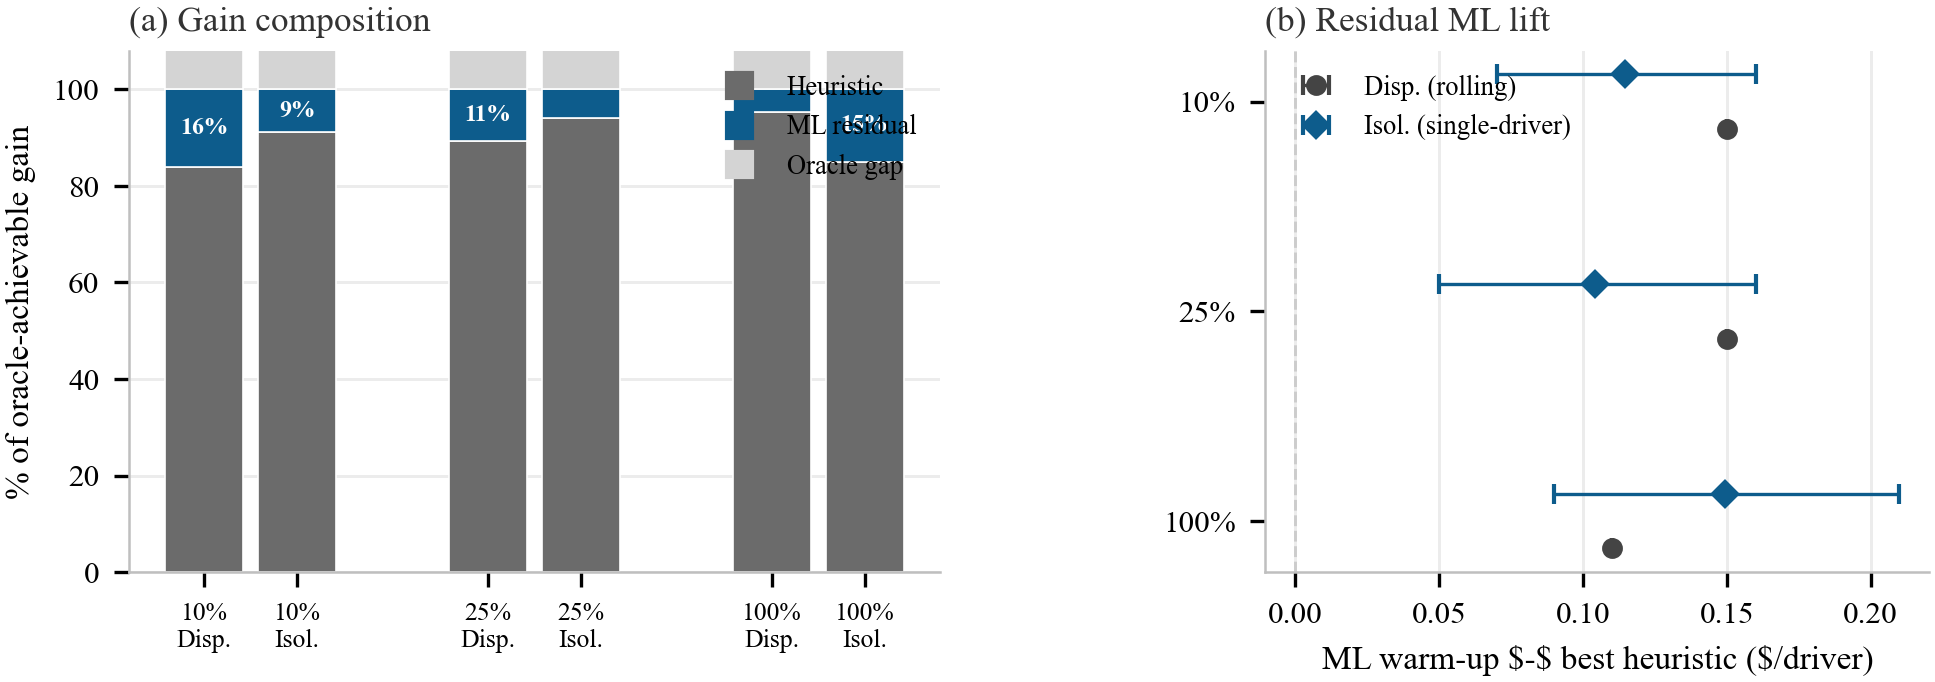
\includegraphics[width=\linewidth]{figures/paper_fig5_single_driver_mechanism.png}
\caption{Route-aware gain decomposition across evaluation layers. \emph{(a)} 100\%-stacked bars showing the composition of oracle-achievable gain at each density and evaluation layer (Disp.\ = rolling dispatch; Isol.\ = controlled single-driver study). Heuristic recovery accounts for 83--95\% of achievable gain; ML residual adds 5--16\%; remaining oracle headroom is small. \emph{(b)} ML warm-up minus best heuristic with 95\% bootstrap intervals, showing the residual ML edge survives at both evaluation layers and all densities.}
\label{fig:single_driver_density}
\end{figure}

This relationship between the two result layers is informative rather than contradictory. The single-driver study confirms that the learned scorer retains a positive paired advantage over the strongest heuristic, but the decomposition also shows that most of the route-aware gain is heuristic recovery in the first place. The dispatch layer then asks whether that residual lift survives under rider exclusivity and shared demand; it does, but only as a modest secondary effect. That is exactly why a dispatch-first paper needs both system-level and controlled analyses.

\subsection{Model Support}
Table~\ref{tab:model_quality} reports Yellow temporal-holdout model quality, and Figure~\ref{fig:model_support} summarizes holdout calibration for the deployed LightGBM scorer. The tuned Yellow model reaches \(R^2=0.801\), RMSE \(=\$5.85\), and 76.1\% route rank-1 accuracy. The tuned Green model reaches \(R^2=0.738\) and RMSE \(=\$2.73\). The MLP edges the Yellow holdout fit slightly with \(R^2=0.804\) and RMSE \(=\$5.81\), while LambdaRank leads rank-1 accuracy at 80.5\% but with substantially weaker absolute fit. We therefore keep tuned LightGBM because it offers the best balance of regression quality and route ranking among the models with usable score calibration. Feature-importance aggregation on the training build attributes about 89\% of total gain to spatial-demand context, 6\% to route geometry, 3\% to landmark proxies, and 2\% to coarse temporal bins, which matches the intended role of the scorer as a corridor- and demand-aware route value model rather than a single-feature shortcut.

\begin{table}[!t]
\caption{Yellow model quality on the March 2015 temporal holdout. January--February 2015 are used for training; March 2015 is used for validation and selection before final retraining on January--March for April policy evaluation.}
\label{tab:model_quality}
\centering
\scriptsize
\setlength{\tabcolsep}{2.5pt}
\begin{tabular}{lrrrr}
\toprule
Model & \(R^2\) & RMSE & Rank-1 & Deployment role \\
\midrule
Ridge (linear) & 0.692 & 6.92 & 68.1\% & Simpler baseline \\
LightGBM (baseline) & 0.786 & 6.02 & 74.2\% & Untuned tree baseline \\
LightGBM (tuned) & 0.801 & 5.85 & 76.1\% & \textbf{Selected scorer} \\
LambdaRank & 0.611 & 7.90 & \textbf{80.5\%} & Ranking-oriented, weak calibration \\
MLP (Neural Net) & \textbf{0.804} & \textbf{5.81} & 74.8\% & Slightly better fit, weaker ranking \\
\bottomrule
\end{tabular}
\end{table}

\begin{figure}[!t]
\centering
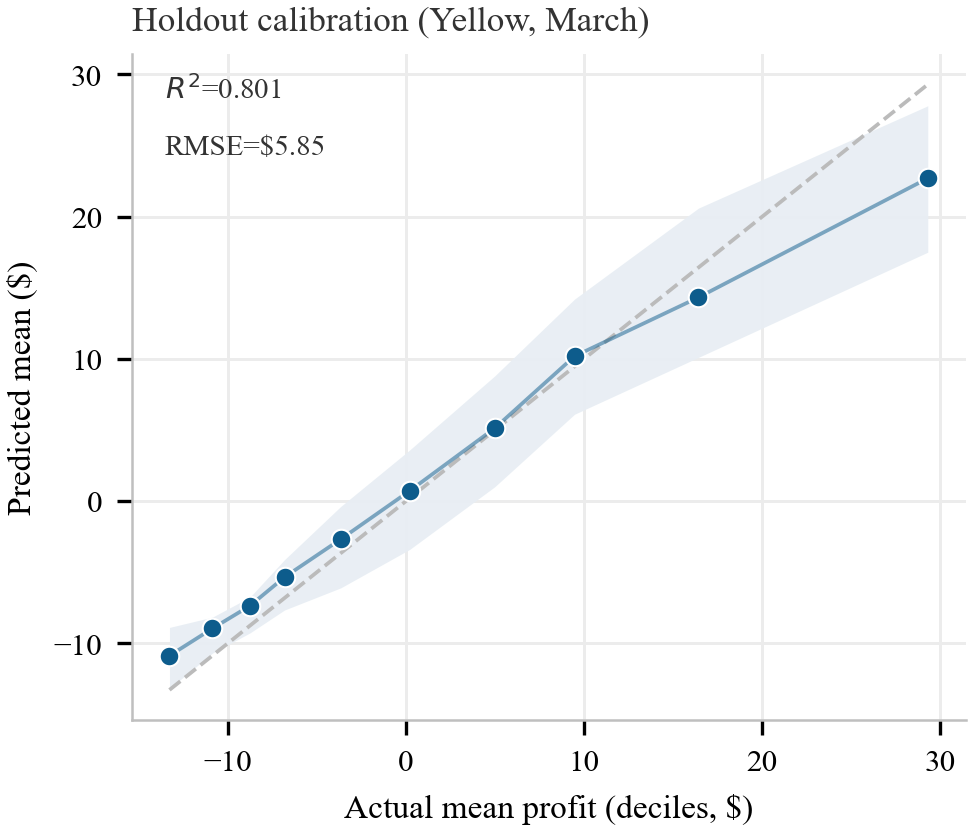
\includegraphics[width=\linewidth]{figures/paper_fig6_model_support.png}
\caption{Holdout calibration for the deployed Yellow LightGBM scorer (March 2015 temporal holdout). Points are decile means of actual versus predicted route profit; the shaded band is the model's interquartile prediction range across routes in each decile. Reported \(R^2\) and RMSE are taken from the model comparison table on the same holdout.}
\label{fig:model_support}
\end{figure}

Figure~\ref{fig:model_support} shows that predicted means track decile-level actual profits on the March holdout without collapsing to a single average, which is the behavior expected of a route scorer used for ranking within a small alternative set. The feature-family breakdown stated above corroborates that the model leans on spatial-demand context rather than on a single proxy family.

\subsection{Sensitivity and Runtime}
Figure~\ref{fig:sensitivity} refines the realism story inside the 10\% stress test. In Yellow dispatch at 10\% density, a tight 2-minute request window with a 2-minute detour yields only \(\$0.36\) of warm-up improvement over cold-start. The primary 5-minute / 4-minute cell yields \(\$0.91\) in the sensitivity grid, consistent with the \(\$0.93\) reported in Table~\ref{tab:dispatch_primary} (the small difference reflects separate seeded runs). A looser 10-minute request window with a 6-minute detour yields \(\$1.36\). Request-window assumptions therefore matter more than moderate detour changes.

\begin{figure}[!t]
\centering
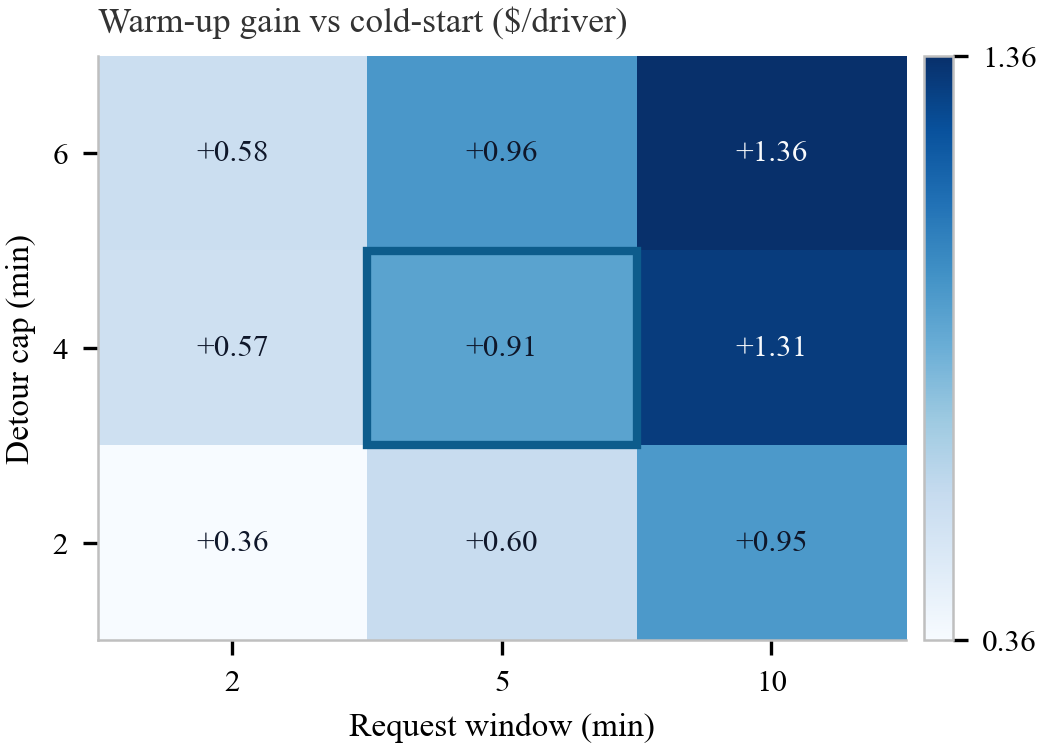
\includegraphics[width=\linewidth]{figures/paper_fig7_sensitivity.png}
\caption{Yellow dispatch sensitivity at 10\% retained-sample density. Each cell reports warm-up improvement over cold-start in scenario profit per launched driver, equivalently the reduction in operating loss. The heatmap shows that request-window assumptions move the dispatch result more than moderate detour relaxation, reinforcing the paper's realism-first claim.}
\label{fig:sensitivity}
\end{figure}

Retrieval geometry also matters. In the single-driver H3 sensitivity, a coarser H3-8 corridor increases warm-up loss to \(\$8.88\), while a wider two-ring corridor reduces it to \(\$4.91\) but lets the strongest heuristic overtake ML by about \(\$0.05\). The corridor definition therefore changes both the candidate pool and the difficulty of the route-ranking problem.

Finally, the dispatch layer is lightweight once the route cache is populated. Table~\ref{tab:runtime} reports mean per-driver evaluation time and mean batch runtime for the primary Yellow dispatch scenario. All four reported policies remain around 17.2--17.4 ms per driver and 36.6--37.1 ms per batch on average.

\begin{table}[!t]
\caption{Primary Yellow dispatch runtime. Times exclude initial route-fetch latency because the simulator runs against the cached route store.}
\label{tab:runtime}
\centering
\scriptsize
\setlength{\tabcolsep}{4.0pt}
\begin{tabular}{lrr}
\toprule
Policy & Mean eval (ms) & Mean batch (ms) \\
\midrule
Cold-start & 17.3 & 36.9 \\
Best heuristic & 17.4 & 37.1 \\
ML warm-up & 17.3 & 36.9 \\
Oracle (route set) & 17.2 & 36.6 \\
\bottomrule
\end{tabular}
\end{table}

\section{Discussion}
The empirical evidence supports three substantive conclusions.

First, route-aware candidate construction materially changes dispatch outcomes. Even after exact request-window filtering and rider exclusivity, the route-aware layer consistently reduces operating loss relative to default cold-start routing in both Yellow and Green. This is the paper's primary systems result: route choice is not merely a navigation detail, but a mechanism that changes which riders are realistically matchable.

Second, learned route ranking is useful but not dominant once strong heuristics are already in place. In the primary Yellow sparse scenario, ML warm-up improves upon the strongest heuristic by only \(\$0.15\) per launched driver; in Green the corresponding margin is \(\$0.27\). The single-driver and dispatch decompositions show why this is not a contradiction: most of the route-aware gain is already recovered by heuristic retrieval and route choice, leaving ML to capture only a smaller residual layer of value.

Third, exact timing is a methodological lever, not a bookkeeping detail. The sensitivity analysis shows that request-window assumptions shift results more than moderate detour relaxation. This implies that ride-pooling studies should distinguish retrieval acceleration tricks from the actual matching rule. In the present implementation, H3 corridors and 15-minute bins narrow the search; exact timestamp compatibility determines which riders remain eligible.

The added path-buffer sanity baseline also sharpens the retrieval claim. A naive 1 km geometric buffer around the route can recover some low-hanging candidate overlap, but it does not approach the matching-ball policies under the same timing and feasibility rules. That gap suggests the main value is not simply ``using more geometry,'' but using route-specific corridor construction that is explicit about both pickup and drop-off compatibility before scoring.

The study nonetheless remains bounded. It is an offline proxy design based on taxi trajectories rather than native pooled requests, so the public benchmark should be read as a controlled test of route-aware candidate construction rather than as an ecological replica of live pooled-demand behavior. The dispatch simulator is rolling-horizon and exclusivity-aware but does not model repositioning or full many-driver global assignment. The public second domain, NYC Green, strengthens robustness but does not substitute for a true second city or restricted operator dataset. The dispatch study uses 1000 drivers and five seeds, which is sufficient for the present comparative evidence but not for a full-scale deployment claim. Finally, the reported losses and loss reductions are scenario-based operating metrics under fixed share and cost assumptions rather than calibrated financial forecasts.

These constraints narrow the paper's scope, but they sharpen its contribution. The paper does not claim that a learned route scorer solves dispatch. It shows, more specifically, that route-aware matching-ball retrieval and exact-time eligibility materially change route-selection conclusions, that those conclusions persist across two public NYC domains, and that strong non-ML heuristics remain the right benchmark for learned ranking in shared dispatch environments.

\section{Conclusion}
This paper presents a dispatch-first evaluation of route-aware warm-up for ride-pooling. The core method is a matching-ball retrieval layer built from H3 corridors, exact request-time filtering, feasibility checks, and route ranking over genuine OSRM alternatives. Embedded inside a rolling-horizon dispatch simulator, that route-aware layer consistently reduces operating loss relative to cold-start routing in the Yellow sparse scenario and preserves the same policy ordering in Green.

The controlled paired study clarifies the mechanism behind the system-level result. Strong heuristics recover most of the route-aware gain in both isolated and shared settings, while learned route ranking contributes a smaller residual improvement. The paper therefore contributes both a route-aware dispatch method and a more disciplined evaluation protocol for judging route-selection policies under realistic timing assumptions.

The immediate implication is methodological as much as operational: ride-pooling studies should not conflate coarse retrieval bins with actual request compatibility, and they should treat route choice as part of candidate construction rather than as a downstream routing detail. Future work can expand this formulation with larger dispatch studies, additional public markets or restricted operational data, and richer many-driver assignment and repositioning logic. Until then, the present evidence supports a narrower but important conclusion: route-aware matching-ball dispatch is worthwhile, exact timing materially matters, and strong heuristics remain the correct benchmark for learned route ranking.

\bibliographystyle{IEEEtran}
\bibliography{references}

\end{document}
